\documentclass{standalone}
\usepackage{tikz}
\begin{document}
    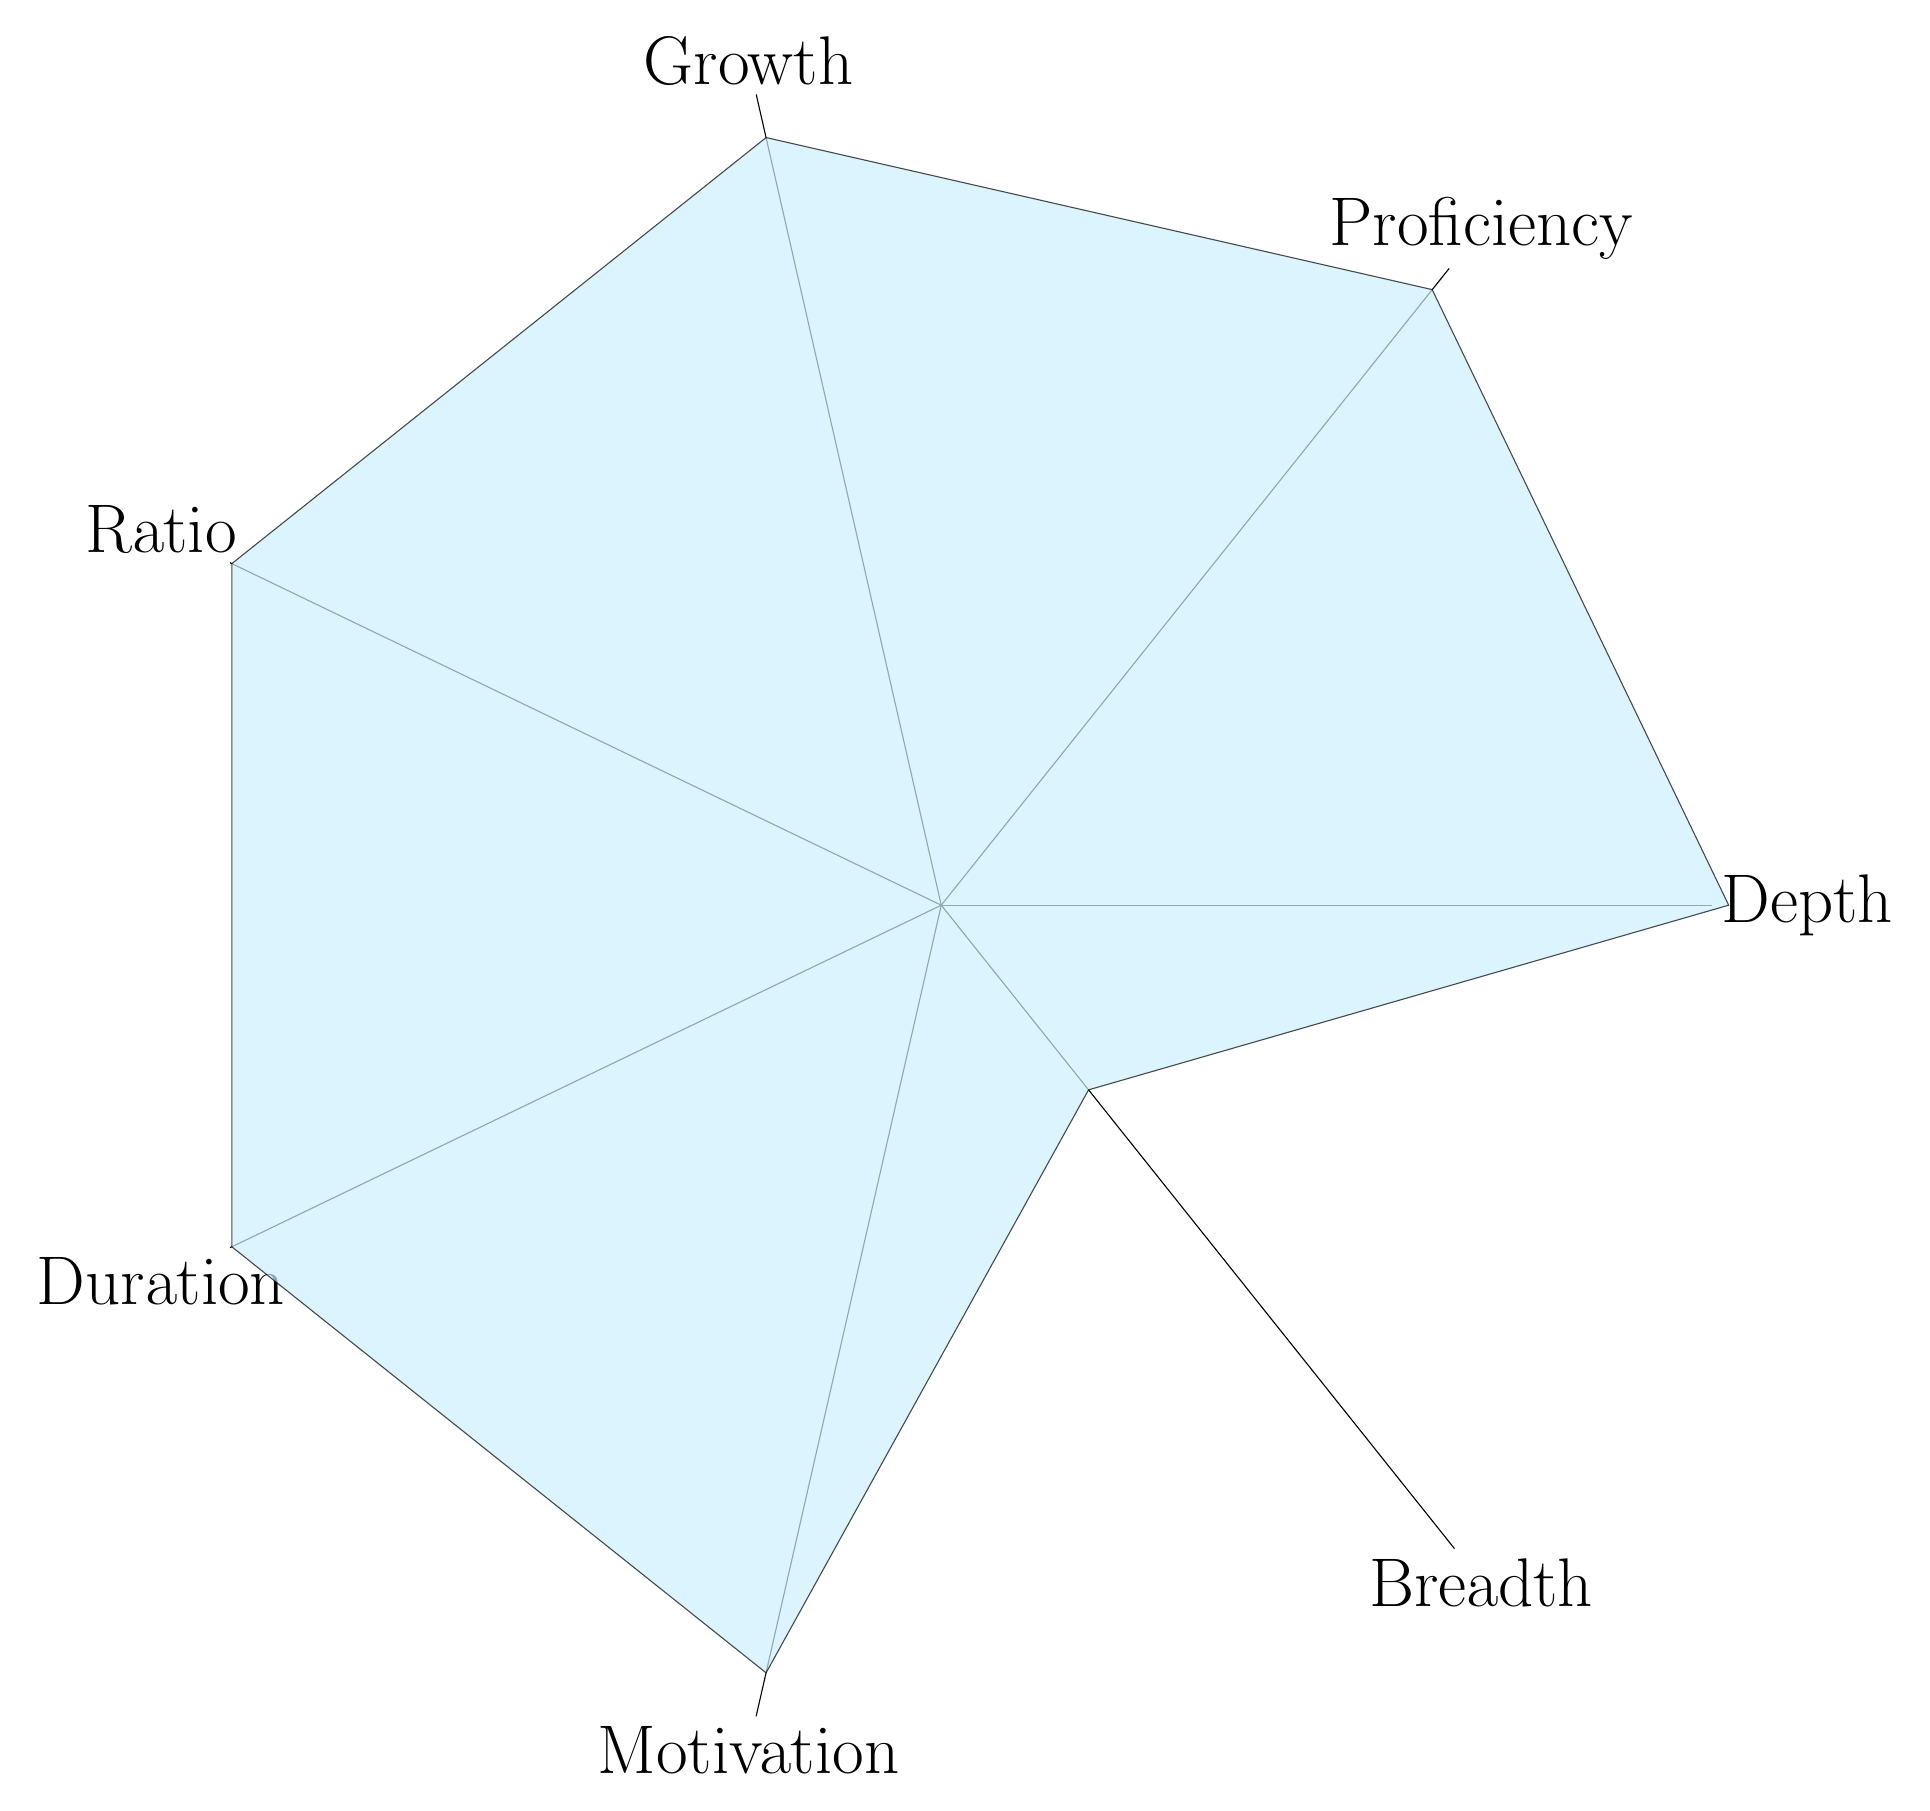
\begin{tikzpicture}
        \coordinate (origin) at (0, 0);

        \foreach[count=\i] \radius/\dim in {10/Proficiency,
                                            10/Growth,
                                            10/Ratio,
                                            10/Duration,
                                            10/Motivation,
                                            3/Breadth,
                                            10/Depth}{
            \coordinate (\i) at (\i * 360 / 7: \radius);
            \node (title) at (\i * 360 / 7: 11) {\Huge\dim};
            \draw (origin) -- (title);
        }

        \draw [fill=cyan!20, opacity=.7] (1)
                                    \foreach \i in {2,...,7}{-- (\i)} --cycle;
    \end{tikzpicture}
\end{document}
